\documentclass[solution, letterpaper]{cs121}

\usepackage{tikz-qtree}
\usepackage{graphicx}
\usepackage{amsmath}

\DeclareMathOperator*{\argmax}{\arg\!\max}

%% Please fill in your name and collaboration statement here.
%\newcommand{\studentName}{Renzo Lucioni and Daniel Broudy}
%\newcommand{\collaborationStatement}{I collaborated with...}
\newcommand{\solncolor}{red}
\begin{document}

\header{5}{April 26, 2013, at 12:00 PM}{}{}

%%%%%%%%%%%%%%%%%%%%%%%%%%%%%%%%%%%%%%%%%%%%%%%%%%%%
\problem{10} %1

\subproblem{} %a
In this problem, our team decides to use a decision theoretic (i.e., greedy) strategy to decide where the dart thrower should aim. We have access to a probability distribution $P$ over the $N$ possible results of a dart throw, given a target $a \in A$, where $A$ is a finite set of targets. We also have access to a utility function $U$ which specifies the value to us of a dart throw result given our current score, which we denote with the random variable $S = s$. For clarity, note that a dart throw result is a certain number of points, and the utility is the \emph{value to us} of that dart throw result. We represent the result of a dart throw aimed at target $a$ with the random variable $R(a) = r_n(a)$, for all $n \in N$. The following equations determine $a^*$, the optimal action given the current score $s$, by adhering to the maximum expected utility (MEU) principle and choosing the action which maximizes the expected utility.

\begin{eqnarray}
\mathbb{E}\left[U(R(a),S)\right] = \sum_{n=1}^N P(r_n(a) | a) U(r_n(a),s) \\
a^* = \argmax_{a \in A} \mathbb{E}\left[U(R(a),S)\right] = \argmax_{a \in A} \sum_{n=1}^N P(r_n(a) | a) U(r_n(a),s)
\end{eqnarray}

\subproblem{} %b
Since the proposed utility function dictates a greedy approach, always preferring larger score reductions to smaller ones, we think the proposed utility function is useful only in a setting where long-term planning is not required. The game of ``301" requires greedy, short-term planning in the early game, where it is best to rack up points quickly, as well as long-term planning in the mid to late game, where it is best to recalculate your ``out" number sequences after each throw in an effort to end the game (i.e., get to 0) as quickly as possible. Note that the latter rarely involves consistently shooting for the largest point values, but instead shooting for a series of smaller numbers which sum to the current score.

A dart player designed using the greedy proposal will only consider the reward for the next, most immediate throw. With the above in mind, we would expect this dart player to make good decisions in the early game, preferring the largest point values it can achieve in an effort to ``get in" (i.e., lower the score) quickly. However, we would expect this dart player to make poor decisions in the mid to late game, since it would be unable to sacrifice short-term gain (i.e., choosing smaller point values) for long-term benefit (i.e., winning the game), continuing to select the largest valued throws possible instead of attempting to string together a series of lesser valued but smarter throws.

\pagebreak

\problem{28} %2

\subproblem{} %a
The \textsc{START\_SCORE}+1 possible game scores in the range [0,\textsc{START\_SCORE}] constitute the states of our MDP model. Meanwhile, each possible (throw at a) \emph{target} on the dartboard constitutes an action in our MDP model.

\subproblem{} %b
Our reward function awards 0 reward to dart throw results (i.e., number of points) over the current score. Dart throw results under the current score are awarded reward equal to their point value. The discount factor, $\gamma$, plays no role in defining our reward function.

\subproblem{} %c
(See {\tt mdp.py} for the completed transition function.)

\subproblem{} %d
We choose to use an infinite rather than finite horizon when finding an optimal policy in the darts scenario because we know that the dart throwing agent will die at some point (i.e., win the game), but we do not have an upper bound on how long it will take for it to end the game and die. In this case, it is possible, albeit extremely unlikely, for the agent to go on living forever, with the game never ending. As such, the agent's total reward might be unbounded, so the problem of maximizing the total reward in a finite number of steps is ill-posed.

\subproblem{} %e
After uncommenting print statements which listed the optimal target given the current state for all states, it appears that the intuition behind the optimal policy resulting from value iteration using the small game is to go for the largest possible point value given the current score in the safest manner possible. That is, in each state (i.e., score) the agent chooses a point value which will get it as close as possible to ending the game. If there are multiple ways to achieve this point value, it seems that the agent chooses the method which will still allow it to make a dent in the score if it misses, as opposed to risking point value higher than the score, in which case the score does not decrease.

\subproblem{} %f
As the discount factor $\gamma$ approaches 1, the agent's optimal policy becomes less intent on winning the game immediately, trying for point values which are not necessarily the largest possible, given the score. When $\gamma \geq 1$, the agent attempts to live forever by always aiming for a miss, since this allows it to accumulate substantial reward indefinitely. When $\gamma$ approaches 0, the agent's optimal policy attempts to end the game as quickly as possible by trying for the largest point values possible, given the score. It seems that the range $0 \leq \gamma \leq 0.5$ is the sweet
% \documentclass[solution, letterpaper]{cs121}

\usepackage{tikz-qtree}
\usepackage{graphicx}
\usepackage{amsmath}

\DeclareMathOperator*{\argmax}{\arg\!\max}

%% Please fill in your name and collaboration statement here.
%\newcommand{\studentName}{Renzo Lucioni and Daniel Broudy}
%\newcommand{\collaborationStatement}{I collaborated with...}
\newcommand{\solncolor}{red}
\begin{document}

\header{5}{April 26, 2013, at 12:00 PM}{}{}

%%%%%%%%%%%%%%%%%%%%%%%%%%%%%%%%%%%%%%%%%%%%%%%%%%%%
\problem{10} %1

\subproblem{} %a
In this problem, our team decides to use a decision theoretic (i.e., greedy) strategy to decide where the dart thrower should aim. We have access to a probability distribution $P$ over the $N$ possible results of a dart throw, given a target $a \in A$, where $A$ is a finite set of targets. We also have access to a utility function $U$ which specifies the value to us of a dart throw result given our current score, which we denote with the random variable $S = s$. For clarity, note that a dart throw result is a certain number of points, and the utility is the \emph{value to us} of that dart throw result. We represent the result of a dart throw aimed at target $a$ with the random variable $R(a) = r_n(a)$, for all $n \in N$. The following equations determine $a^*$, the optimal action given the current score $s$, by adhering to the maximum expected utility (MEU) principle and choosing the action which maximizes the expected utility.

\begin{eqnarray}
\mathbb{E}\left[U(R(a),S)\right] = \sum_{n=1}^N P(r_n(a) | a) U(r_n(a),s) \\
a^* = \argmax_{a \in A} \mathbb{E}\left[U(R(a),S)\right] = \argmax_{a \in A} \sum_{n=1}^N P(r_n(a) | a) U(r_n(a),s)
\end{eqnarray}

\subproblem{} %b
Since the proposed utility function dictates a greedy approach, always preferring larger score reductions to smaller ones, we think the proposed utility function is useful only in a setting where long-term planning is not required. The game of ``301" requires greedy, short-term planning in the early game, where it is best to rack up points quickly, as well as long-term planning in the mid to late game, where it is best to recalculate your ``out" number sequences after each throw in an effort to end the game (i.e., get to 0) as quickly as possible. Note that the latter rarely involves consistently shooting for the largest point values, but instead shooting for a series of smaller numbers which sum to the current score.

A dart player designed using the greedy proposal will only consider the reward for the next, most immediate throw. With the above in mind, we would expect this dart player to make good decisions in the early game, preferring the largest point values it can achieve in an effort to ``get in" (i.e., lower the score) quickly. However, we would expect this dart player to make poor decisions in the mid to late game, since it would be unable to sacrifice short-term gain (i.e., choosing smaller point values) for long-term benefit (i.e., winning the game), continuing to select the largest valued throws possible instead of attempting to string together a series of lesser valued but smarter throws.


\problem{28} %2

\subproblem{} %a
The \textsc{START\_SCORE}+1 possible game scores in the range [0,\textsc{START\_SCORE}] constitute the states of our MDP model. Meanwhile, each possible (throw at a) \emph{target} on the dartboard constitutes an action in our MDP model.

\subproblem{} %b
Our reward function awards 0 reward to dart throw results (i.e., number of points) over the current score. Dart throw results under the current score are awarded reward equal to their point value. The discount factor, $\gamma$, plays no role in defining our reward function.

\subproblem{} %c
(See {\tt mdp.py} for the completed transition function.)

\subproblem{} %d
We choose to use an infinite rather than finite horizon when finding an optimal policy in the darts scenario because we know that the dart throwing agent will die at some point (i.e., win the game), but we do not have an upper bound on how long it will take for it to end the game and die. In this case, it is possible, albeit extremely unlikely, for the agent to go on living forever, with the game never ending. As such, the agent's total reward might be unbounded, so the problem of maximizing the total reward in a finite number of steps is ill-posed.

\subproblem{} %e
After uncommenting print statements which listed the optimal target given the current state for all states, it appears that the intuition behind the optimal policy resulting from value iteration using the small game is to go for the largest possible point value given the current score in the safest manner possible. That is, in each state (i.e., score) the agent chooses a point value which will get it as close as possible to ending the game. If there are multiple ways to achieve this point value, it seems that the agent chooses the method which will still allow it to make a dent in the score if it misses, as opposed to risking point value higher than the score, in which case the score does not decrease.

\subproblem{} %f
As the discount factor $\gamma$ approaches 1, the agent's optimal policy becomes less intent on winning the game immediately, trying for point values which are not necessarily the largest possible, given the score. When $\gamma \geq 1$, the agent attempts to live forever by always aiming for a miss, since this allows it to accumulate substantial reward indefinitely. When $\gamma$ approaches 0, the agent's optimal policy attempts to end the game as quickly as possible by trying for the largest point values possible, given the score. It seems that the range $0 \leq \gamma \leq 0.5$ is the sweet spot for creating this strictly greedy behavior. Common across all optimal policies are an apparent preference for the outer ring of the board, as well as the fact that the game eventually ends.

\problem{25} %3

\subproblem{} %a
DANBRO

\subproblem{} %b
DANBRO

\subproblem{} %c
By (A), we know that if policy iteration terminates, it terminates with the optimal stationary policy. By (B), we know that the policy improves or stays that same after each iteration phase (i.e., every step the policy improves). This means that a given policy can be encountered at most once. Since there are a finite number of states and actions, there are a finite number of policies. Therefore, we must terminate by the time we have iterated through the finite number of policies. Therefore, policy iteration always terminates with an optimal stationary policy (assuming the policy space is convex).


\problem{30} %4

\subproblem{} %a
We implemented the $\varepsilon$-Greedy and Boltzmann action selection strategies for balancing exploration and exploitation. See {\tt model based.py} for our implementations.

\subproblem{} %b
DANBRO

\subproblem{} %c
DANBRO



\end{document} 
spot for creating this strictly greedy behavior. Common across all optimal policies are an apparent preference for the outer ring of the board, as well as the fact that the game eventually ends.

\problem{25} %3

\subproblem{} %a
%DANBRO
% question: are we in an infinite horizon case? and if not how does that effect our assumptions in this proof
The following will be a proof that if policy iteration terminates with a policy $\pi^*$, then $\pi^*$ is an optimal stationary policy. For this proof we will discuss a Bellman operator on the values from one round to the next of policy iteration. We will then quote the Lecture 19 notes and other sources to demonstrate that the operator is a contraction. When an operator is a contraction, then we always have unique fixed point. In the case of this proof, the unique fixed point is a vector of values for each state. This unique vector of values also determines the unique optimal policy vector that will cease to update the $\pi$'s and trigger the unique case in which policy iteration terminates, so it converges on the optimal stationary policy.  

Let's see how policy iteration works. We first initialize our policies to something random. We then define a system of equations with the equation
\[ V^{\pi}(s)  =  \left[ R(s,\pi(s) ) + \gamma \sum_{s'} P(s' | s,\pi(s))V(s')\right ]\]
where the $\pi$ is the the policy that we already have (which by definition is a mapping from states to actions). Solving this system of equations gives us an approximation for the value of a state. We will think of this as $V(s)$.
Then for each state, we evaluate the new value of a state action pair $Q(s,a)$ and select the action $a$ that maximizes $Q$ for a given state. This action $a$ is our new new $\pi$ for that state. This is summarized by the following equation:
\[\pi^{new} = \argmax_{a \in A}  \left[ R(s,a ) + \gamma \sum_{s'} P(s' | s,a)V^{new}(s')\right ]\]
We then repeat this process until the $\pi$ values cease to change. (We of course do not repeat the step of setting the $\pi$'s to random values.) \\

Now that we have a well defined situation, I think the easier way to go about proving this problem converges to an optimal policy is to prove a contraction over the $V$'s that we associate with each state from round to round.  In this problem we are operating with an infinite horizon. As stated in the Lecture 19 notes, when we are in an infinite horizon case there exists an optimal solution that is a stationary policy where you will always take the same action $\pi(s)$ at state $s$.  If we can prove that the $V$'s converge to some fixed values it will hold that the $\pi$'s will converge to a fixed value as well, because as the $V$'s stop changing the rule to update the $\pi$s will be unchanged and we will have terminated at our unique fixed point. How do we prove that the $V$'s are converging to a unique fixed point? We conclude this by identifying that, much like in value iteration, we are working with a Bellman operator.\\

For policy iteration we define the following Bellman optimality operator: $\tau : R^N \rightarrow R^N$ for any vector $V \in R^N$
\[(\tau V)(s) = \argmax_{a \in A}  \left[ R(s,\pi(s) ) + \gamma \sum_{s'} P(s' | s,\pi(s))V(s')\right ]\]

The Bellman optimality operator has the property that if from one iteration to the next the $V$ is left unchanged, then we have terminated at a fixed point of the Bellman optimality operator $\tau$ which by definition is unique due to the contraction property of $\tau$.
From the notes on Lecture 19, a more formal definition of the contraction property that is satisfied by the Bellman operator is \[ ||\tau(V_1) - \tau(V_2) || \leq \gamma || V_1 - V_2 ||, \text{ for } \gamma \in [0,1)\]

Much as in value iteration, this Bellman operator $\tau$ is an operation on the space of value functions. For the optimal value function, $V^* = \tau(V^*)$. In policy iteration, although it is the policy $\pi$ that we are iterating and that we care about, each round produces a new $V$ that behaves much like value iteration. We solve for our new $V$'s and the pick the optimal $\pi$s and repeat. By picking the optimal $\pi$'s, we are effectively taking the $\argmax$ over $a$ of the $V^{\pi}$ because we use the $\pi$ that was optimized in the previous iteration. From the definition of a Bellman equation, we can conclude that if we terminate at a fixed solution for $V$'s then we have terminated at the optimal solution for the $V$'s. Now that we know the $V$'s converge to a fixed point that is optimal we can also conclude that the $\pi$'s converge to a fixed solution that is optimal as well, because the updating of the $\pi$'s is based on the $V$'s and optimizing the $V$'s can only increase the value of the $\pi$'s, which increases the utility we get from following the fixed policy $\pi^*$. In the end, we can conclude that if policy iteration terminates with a policy $\pi^*$, then $\pi^*$ is an optimal stationary policy. 

\subproblem{} %b
%DANBRO
We would now like to prove that if $\pi^{(1)}$ is the policy before an iteration  phase and $\pi^{(2)}$ is the policy after the phase, then for every state $s$, 
\[ V^{\pi^{(2)}} (s) \ge V^{\pi^{(1)}}(s) \]

We will first show that this holds true for some state $\hat{s}$ when $\hat{s}$ is the only state in which the action is changed (i.e., improved). We will then convince ourselves that it holds to be true, by symmetry, for all states.  

We begin with a proof by contradiction. Assume that  $V^{\pi^{(2)}} (\hat{s}) < V^{\pi^{(1)}}(\hat{s})$. We are discussing the case where the only policy that changed between  $\pi^{(1)}$ and $\pi^{(2)}$ was $\pi^{(2)}(\hat{s})$. In state $\hat{s}$ we must have evaluated a $Q(s,a)$ and picked the action $\argmax$ over $a$ that maximized our $Q$ in state $\hat{s}$. If in fact we picked the best action available to us in state $s$ our value cannot go down, else we would have picked the previous action again and $V^{\pi^{(2)}} (\hat{s}) = V^{\pi^{(1)}}(\hat{s})$ would be the case. It is always an option to select the action you had before and because we are assuming in this case that $\hat{s}$ is the only one that is changing we could chose to have nothing change so the values would definitely not go down. You would not change your action for the worse. Therefore, it is impossible for the statement $V^{\pi^{(2)}} (s) < V^{\pi^{(1)}}(s)$ to be true in this limited case. Changing our action can only improve the value associated with the current state.
\[\pi^{new} = \argmax_{a \in A}  \left[ R(s,a ) + \gamma \sum_{s'} P(s' | s,a)V^{new}(s')\right ]\] 

Now we have established that no state is going to change its individual policy for the worse on its own. Although more than just the current state can change its policy in a given round of policy iteration, we know that all states are only going to change their policy (the action they take when in state $s$) in a way that makes their current state have a greater or equal value. 
Again, assume for the purposes of contradiction that $V^{\pi^{(2)}} (\hat{s}) < V^{\pi^{(1)}}(\hat{s})$. If this were true, then you could have picked the action you picked before policy iteration changed that caused it to select the action with the lesser value. You can then see that by symmetry, all other actions that ended up with their value decreasing due to a new policy would have instead just picked the same policy as the previous round and would not have selected the policy that made their value decrease. In this manner, we see that the only policy changes that remain are the ones that improve their value from one round to the next. It is also important to note that the value of state increasing from one round to the next (by virtue of a better action selection) can only have a positive impact on the other values associated with states in that new round because all states can now transfer into the state that has a higher value with some probability. 

Now we finally see the full picture: you will never update your $\pi^1 \rightarrow \pi^2$ if the $\pi^2$ makes you worse off. Other states updating their $\pi^1 \rightarrow \pi^2$ in a way that increases that state's value can only have a positive effect on other values by increasing the value of the sum across all the states you can move into. Thus, \[ V^{\pi^{(2)}} (s) \ge V^{\pi^{(1)}}(s) \]

\subproblem{} %c
By (A), we know that if policy iteration terminates, it terminates with the optimal stationary policy. By (B), we know that the policy improves or stays that same after each iteration phase (i.e., every step the policy improves). This means that a given policy can be encountered at most once. Since there are a finite number of states and actions, there are a finite number of policies. Therefore, we must terminate by the time we have iterated through the finite number of policies. We can hence say that policy iteration always terminates with an optimal stationary policy.

We can restate this as follows. We know from (A) that if we stop changing the policy function then we are at the optimum strategy. We also know there are a finite number of strategies because there are a finite number of states and actions. We also know from (B) that we will only improve through iterations of policy changes. So if we can only stop at the optimum, we are always moving towards the optimum and there is a finite number of places we could be, and therefore we are guaranteed to converge at the optimum.


\problem{30} %4

\subproblem{} %a
We implemented time-$T$ mode switching and $\varepsilon$-Greedy strategies for balancing exploration and exploitation. See {\tt modelbased.py} for our implementations. The following graph show, for both exploration/exploitation strategies, the relationship between performance (average number of throws to complete a game) and epoch size used to update the optimal policy. Epoch sizes of 3, 10, and 100 were used. 

\begin{center}
%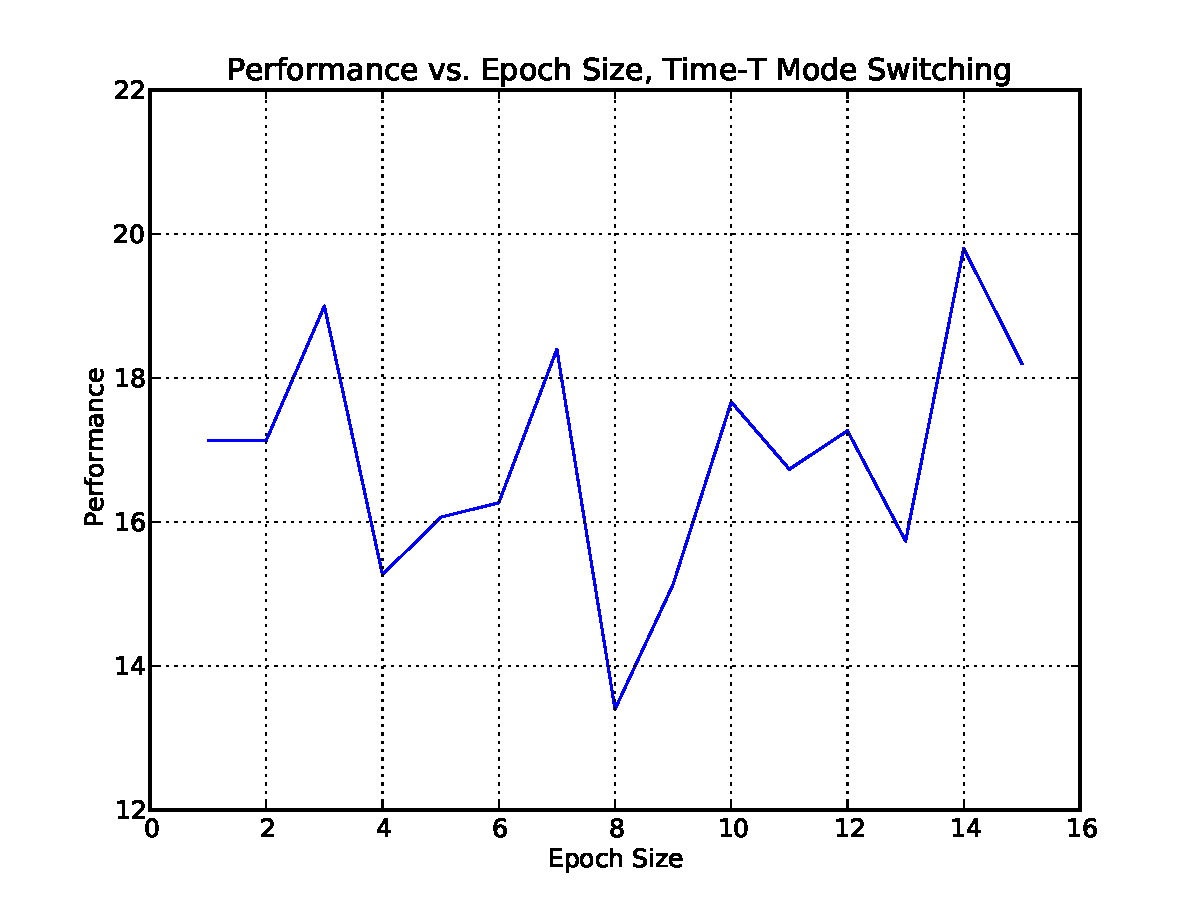
\includegraphics[scale=0.8]{source/perf-v-epoch-mode-switch.pdf}
%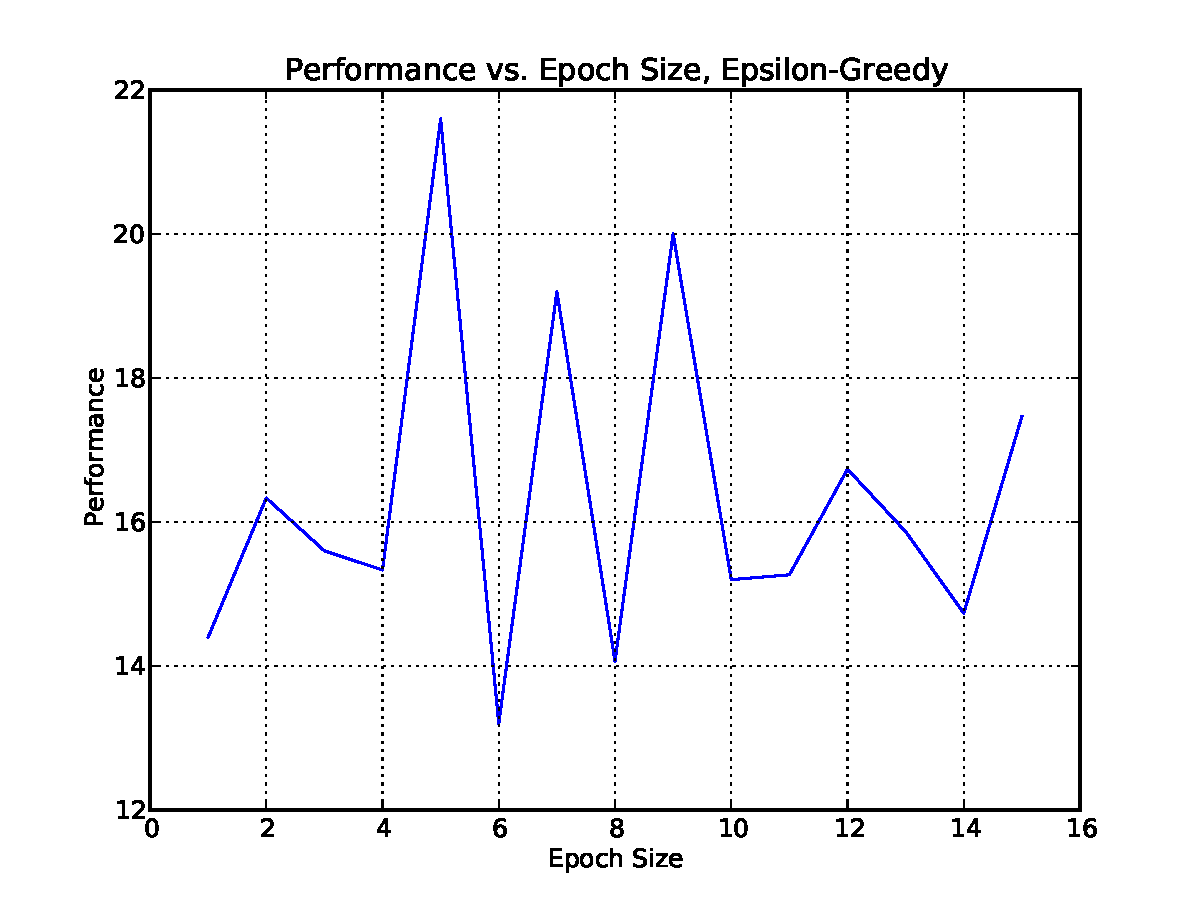
\includegraphics[scale=0.8]{source/perf-v-epoch-greedy.pdf}
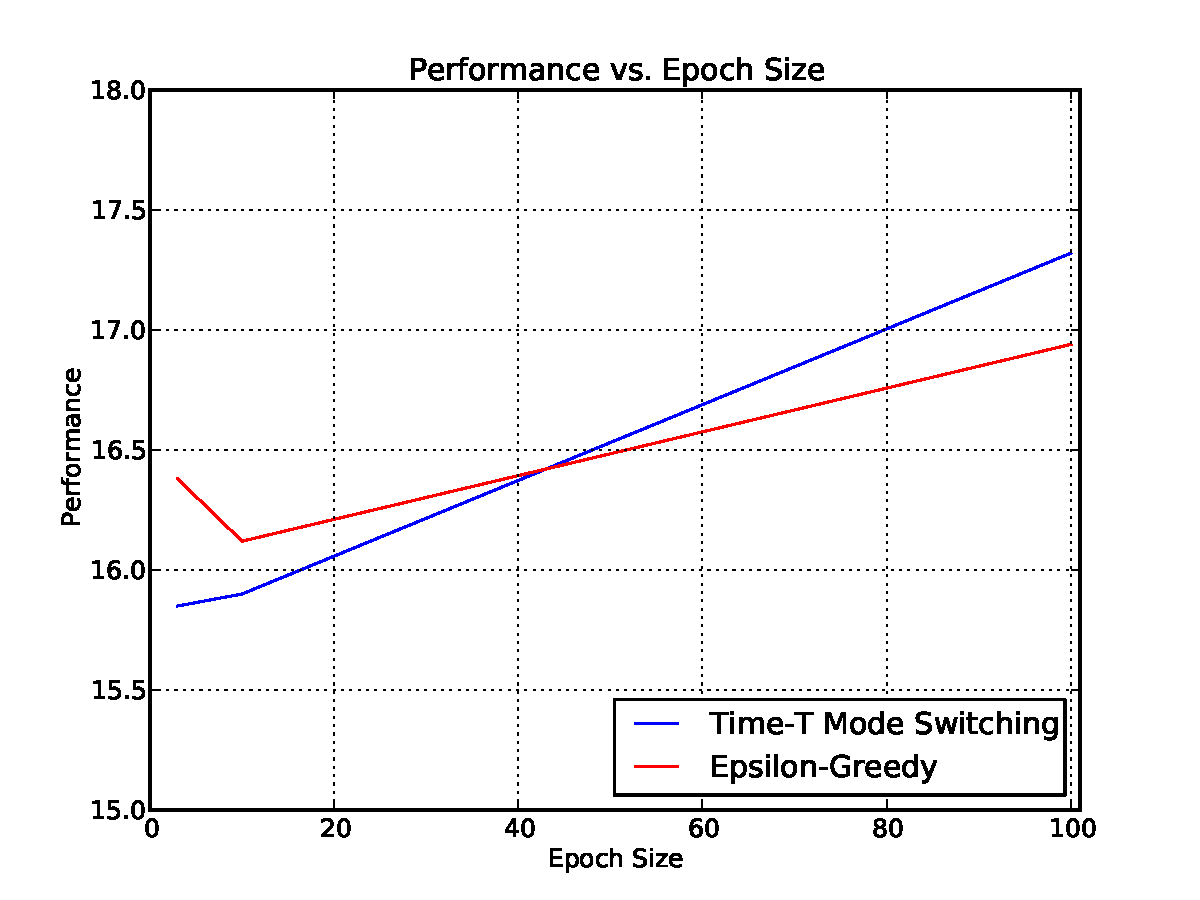
\includegraphics[scale=0.8]{source/perf-v-epoch-size.pdf}
\end{center}

By studying the graph, we see that an epoch of size approximately 10 is correlated with the best performance (i.e., the lowest average number of throws to complete a game). The graph shows that while the time-$T$ mode switching and $\varepsilon$-Greedy strategies are similar in terms of performance, the time-$T$ mode switching strategy performs better in a situation where the epoch size is about 10. This makes sense, since completing a game on the medium-size board seems to take an average of 20 turns. This means that with an epoch size of 100, the policy will be updated much less frequently. 

\subproblem{} %b
DANBRO

\subproblem{} %c
DANBRO



\end{document}